%(M5-M24) (Leader: NUIDUCD-CeADAR, support: NCSR
%"D", FDI, Fraunhofer, INRIA)
\subsection{Introduction} \label{introduction}
Considering the AI efficiency dimension of the MANOLO project, tackling this task from the data perspective will involve the development of, among other techniques, Dataset Distillation (DD) methods. These would aim to create compact, high-fidelity data summaries from large datasets while retaining essential data patterns and dynamics. This DD functionality is critical for achieving MANOLO's project goals of improved efficiency, as well as the mitigation of ethical issues. This is in response to a clear trend in AI of model and dataset size growth. Compare the 3.2 million image size of the Imagenet dataset \cite{imagenet} from 2009, with the 5.85 billion images of 2022's LAION-5B dataset \cite{laion}, integral to the training of many popular image generation models, such as Stable Diffusion. Similarly, the Imagen generative model is trained on 15 billion images \cite{imagen}, while ChatGPT's GPT4 was trained on 499 billion tokens of text data \cite{guimaraes2024pre}. While this massive growth has enabled new applications and capabilities for AI, it has also brought upon a number of problematic implications in the dimensions of efficiency and ethics. Current training processes used for  AI language models such as ChatGPT have significant energy requirements, rivaling the annual consumption of hundreds of American households \cite{energyhouseholds}, contributing to greenhouse gas emissions. Additionally, large datasets are hard to accommodate on hardware with limitations on power consumption, storage capacity, and network bandwidth, such as edge devices. With respect to the ethical implications, the costs associated with large models and datasets may present a barrier to entry for smaller organizations and teams, which could in turn contribute to the monopolization of AI technologies. DD represents one technique that could be used by AI researchers to alleviate these challenges.

The most widely studied approaches to DD can be categorized into Data Matching and Meta-Learning \cite{dd_survey}. Data Matching aims to match the statistical properties of a model that is trained on a distilled dataset with those of a model that is trained on the original, non-distilled dataset. Different techniques in the Data Matching field include Gradient Matching, Trajectory Matching, and Distribution Matching. While this approach has achieved state-of-the-art performance in many DD tasks \cite{datadam}, it involves the use of computationally expensive optimization due to its iterative nature, particularly across long training periods or large parameter spaces. In addition to this drawback, Data Matching has limitations with respect to different computational architectures. For instance, Gradient Matching requires the computation of the gradient of the loss function of the model trained on the distilled data in order to compare it with that of the model trained on the original data. This is incompatible with neuromorphic computing paradigms, where the incoming data is in the form of discrete spike trains, and as such, their gradient cannot be precisely calculated \cite{bengio2013estimating}. Other works make use of meta-learning approaches to DD, particularly back-propagation through time (BPTT) and Kernel Ridge Regression (KRR). However, both of these approaches also suffer from scalability issues, in the case of BPTT due to the high computational overload of unrolling the recursive computation graph across long trajectories, and in the case of KRR due to inefficiencies in kernel computation \cite{dd_survey}.

In the following sections, we outline our efforts towards the development of a novel, clustering-based DD approach. This method differs from the traditional DD approaches described above by performing the distillation task not on the original data, but rather on the data's encodings in the latent space of a variational autoencoder (VAE) trained on the original dataset. We have initially evaluated the technique on two image datasets due to time constraints, and future research efforts will focus on testing its validity for other modalities, as well as on improving the distillation performance.

\subsection{Clustering-Based DD}\label{subsec:2.3_datdist_tech1}

One of the key goals of the MANOLO project is to enable efficient training and deployment of AI models across the Cloud-Edge Continuum (CEC), where computational resources are often constrained. This is where DD can align with MANOLO’s efficient AI goals by creating reduced datasets which preserve essential information, thus ensuring faster, lower-memory, and resource-efficient model training. Furthermore, since MANOLO’s techniques are intended for use with diverse data types, DD with agnostic techniques (e.g., clustering) will help standardise the data preparation activity across various use cases. As such, particular attention was given to developing a DD technique that would be modality-agnostic.

\subsubsection{Methodology}

Our research into DD focused on distilling computer vision datasets, namely MNIST and CIFAR10. The MNIST dataset is a collection of 70,000 grayscale images of handwritten digits (0–9), while the CIFAR-10 dataset consists of 60,000 color images across 10 distinct classes (e.g., animals, vehicles). These datasets are commonly used for training and testing in image classification tasks.

Our proposed DD methodology uses a combination of Variational Autoencoders (VAEs) and K-means clustering to reduce the size of computer vision datasets while maintaining high accuracy metrics when used for classification tasks. Variational Autoencoders are neural networks that encode input data into a compressed latent space, which captures the data's essential features. A peripheral benefit of training VAEs for use in DD is their potential to  be used for data synthesis. This is done by sampling values from the latent space, then subsequently generating new datapoints from the conditional distribution of the data given the latent variable \cite{8285168}. This further aligns with the MANOLO project's efficiency goals, as it allows for the solution of two different tasks, DD and dataset generation, with the same technique.

In our approach, we train a Variational Autoencoder on the dataset in order to generate a latent space. The latent dimension used for the MNIST dataset is 15, and the one used for the CIFAR-10 dataset is 100 due to its additional complexity. After this, the latent space is clustered into N clusters, where N is the number of target classes in the dataset being distilled. Since the number of clusters are pre-determined, the clustering algorithm used to achieve this is K-means \cite{hartigan1979algorithm}. Using this algorithm has a number of advantages in the context of MANOLO's project goals, specifically computational efficiency superior to that of more complex DD methods, low memory overhead on edge devices, and ease of implementation due to its availability in standard ML libraries. Figure \ref{fig:umap-mnist} shows a visualization of the K-means clustered latent space for the MNIST image dataset, generated using the UMAP dimensionality reduction technique \cite{mcinnes2018umap}. Once the clustering process is complete, the centroid of each cluster is calculated, and the distances from each dataset sample encoded in the latent space to its corresponding cluster centroid are found. The measure used to calculate this is Euclidean distance. 

\begin{figure}
    \centering
    \caption{UMAP visualization of the K-Means clustered latent space of the MNIST dataset}
    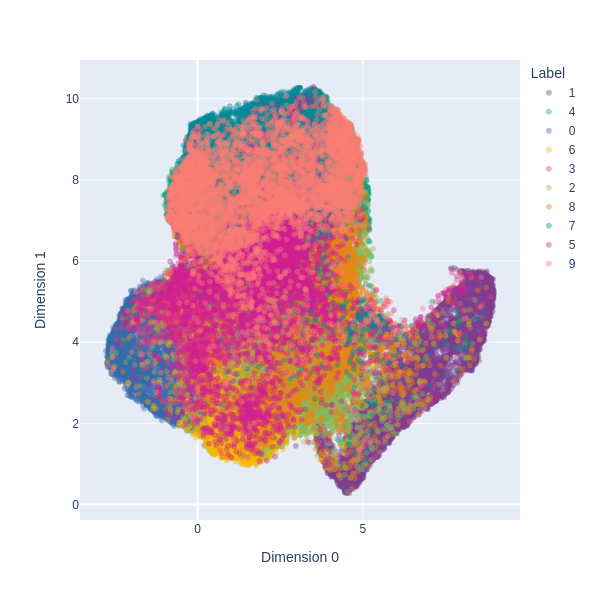
\includegraphics[width=1\linewidth]{fig_datadistill/newplot.png}
    % \caption{UMAP visualization of the K-Means clustered latent space of the MNIST dataset}
    \label{fig:umap-mnist}
\end{figure}

In order to distill the clustered dataset, the Euclidean distances from each encoded sample to its corresponding cluster centroid was found. The samples with the shortest distance to their centroid were then removed from the dataset. The logic behind this is that these samples are the easiest to classify and contribute the least amount of information to the training process, so their removal from the dataset will not adversely affect model performance. In addition to this, we also removed samples that were furthest from their cluster centroids, as well as randomly selected samples. This was done in order to gain more insight into how this DD method affected underlying data structures.

To examine the effects of our clustering-based DD method on the accuracy of classification tasks, a ResNet-50 classifier was trained on the MNIST and CIFAR-10 image dataset for a total of 50 and 200 epochs respectively. The classifier was trained on a number of different distillation levels, from 10\% to 90\%, and the test set accuracy was evaluated for each different level. This was done to investigate the trade-off between DD and classification accuracy. A base classifier was also trained in each dataset's case with a distillation of 0\% for comparison purposes.

\subsubsection{Results}

%
\begin{table}[ht]
    \centering
    \caption[Comparison of ResNet-50 classifier accuracies]{Comparison of ResNet-50 classifier accuracies for the MNIST dataset at distillation proportions between 10\% and 90\%. Baseline classifier accuracy is shown at a distillation of 0\%.}
    \begin{tabular}{|c|c|c|c|c|c|c|}
        \hline
&  \multicolumn{6}{|c|}{\textbf{Accuracy (\%)}} \\ \hline
& \multicolumn{3}{|c|}{\textbf{MNIST}} &
       \multicolumn{3}{|c|} {\textbf{CIFAR-10}}\\ 
        \hline 
        
        \textbf{Distillation (\%)} &  Random & Nearest & Furthest & Random & Nearest & Furthest \\ 
        \hline
        
        0 & 99.08 & 98.90 & 98.97  & 90.60 & 90.09 & 90.09 
         \\   \hline
        
        10 & 98.81  &  98.78 & 98.95 & 89.42 & 89.40 & 89.91
         \\   \hline

        20 & 98.78 & 98.77 & 98.82 & 88.59 & 88.70 & 88.79
        \\  \hline
        30 & 98.71 &  98.79 & 98.78 & 88.29 & 87.77 & 88.06
        \\    \hline
        40 & 98.83 & 98.71 & 98.89 & 87.65 & 87.63 & 87.04
        \\    \hline
        50 & 98.41 & 98.51 & 98.57 & 86.02 & 85.90 & 85.55
        \\    \hline
        60 & 98.54 & 98.30 & 98.31 & 84.67 & 84.47 & 84.78 
        \\    \hline
        70 & 98.08 & 97.93 & 98.09 & 82.59 & 81.39 & 80.70 
        \\    \hline
        80 & 97.18 & 97.53 & 97.48 & 71.52 & 78.19 & 75.59 
        \\    \hline
        90 & 96.31 & 96.45 & 96.25 & 52.88 & 56.36 & 61.53
        \\   \hline
    \end{tabular}
    % \caption[Comparison of ResNet-50 classifier accuracies]{Comparison of ResNet-50 classifier accuracies for the MNIST dataset at distillation proportions between 10\% and 90\%. Baseline classifier accuracy is shown at a distillation of 0\%.}
    \label{tab:dataset_distillation_results}
\end{table}
%

In this section, we present the results of our experiments on how Clustering-Based DD affects the performance of ResNet-50 classifiers trained on the MNIST and CIFAR-10. Table \ref{tab:dataset_distillation_results} presents the accuracy of each ResNet-50 classifier trained on the MNIST dataset after 50 epochs. When removing the nearest samples to each cluster centroid, the drop in accuracy as the distillation increases is small, with the classifier trained at 90\% distillation only performing 2.45\% worse than the baseline model in terms of accuracy on the test set. Similar metrics can also be observed for the Random and Furthest removal criteria. However, it is worth noting that ResNet-50 is a deep model with 50 layers, and the MNIST dataset is simple, with low variability, so even with a very small amount of data it is expected that the classifier will perform well.

\begin{figure}
    \centering
    \caption[Accuracy on MNIST using sample removal on nearest distance to cluster centroid]{Accuracy over Epochs of training for ResNet-50 Classifiers trained on the MNIST dataset with different levels of Clustering-Based DD. The removal criterion used was Nearest distance to cluster centroid.}
    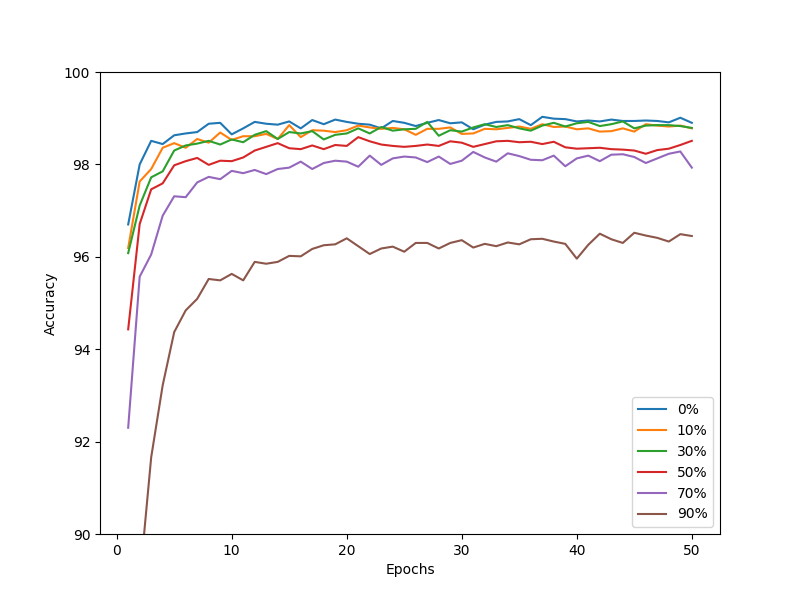
\includegraphics[width=1\linewidth]{mnist_results.png}
    % \caption{Accuracy over Epochs of training for ResNet-50 Classifiers trained on the MNIST dataset with different levels of Clustering-Based DD}
    \label{fig:mnist_results_dd}
\end{figure}

Figure \ref{fig:mnist_results_dd} shows the accuracy of the ResNet-50 classifier on the MNIST dataset at different distillation levels. In order to preserve the visual clarity of the line chart, only a subset of tested distillation levels are presented. We noticed an interesting pattern in our experimental results where performance tended to group into distinct clusters. One can see in Table \ref{tab:dataset_distillation_results} that the accuracy at a distillation of 0\% and that at 80\% is fairly similar, while the accuracy at a distillation of 90\% is significantly lower. Table \ref{tab:dataset_distillation_results} shows experimental results for our DD method on the CIFAR-10 image dataset after 200 epochs of training. The overall performance here is lower than on the MNIST image dataset due to CIFAR-10's multi-channel nature, higher complexity, and increased variability. Similar to the MNIST results presented in Table \ref{tab:dataset_distillation_results} and Figure \ref{fig:mnist_results_dd}, we can observe two distinct performance clusters with the CIFAR-10 dataset. As distillation levels increase from 0\% to 80\%, there is an accuracy drop of less than 12\%, but when the distillation level is 90\%, the accuracy drops by 33.73\% when compared to the baseline. This sudden drop in accuracy can also be observed in Figures \ref{fig:cifar_results_nearest}, \ref{fig:cifar_results_furthest}, and \ref{fig:cifar_results_random}, which show the test accuracy over epochs of training for the CIFAR-10 classifiers using the 3 different DD removal criteria - Nearest, Furthest, and Random. This pattern is worth investigating in future research as it could potentially indicate the existence of a consistent elbow point for our Clustering-Based DD method across multiple datasets. It is also worth noting that the distance criterion used to distill the data had an effect on the accuracy of the classifier. From Table \ref{tab:dataset_distillation_results} we can see that at a distillation levels of 80\% and 90\%, the performance of the CIFAR-10 classifier is lowest when points are removed randomly, as opposed to removing samples nearest or furthest from their respective cluster centroid. 




\begin{figure}
    \centering
    \caption[Accuracy on CIFAR-10 using sample removal on nearest distance to cluster centroid]{Accuracy over Epochs of training for ResNet-50 Classifiers trained on the CIFAR-10 dataset with different levels of Clustering-Based DD. The removal criterion used was Nearest distance to cluster centroid.}
    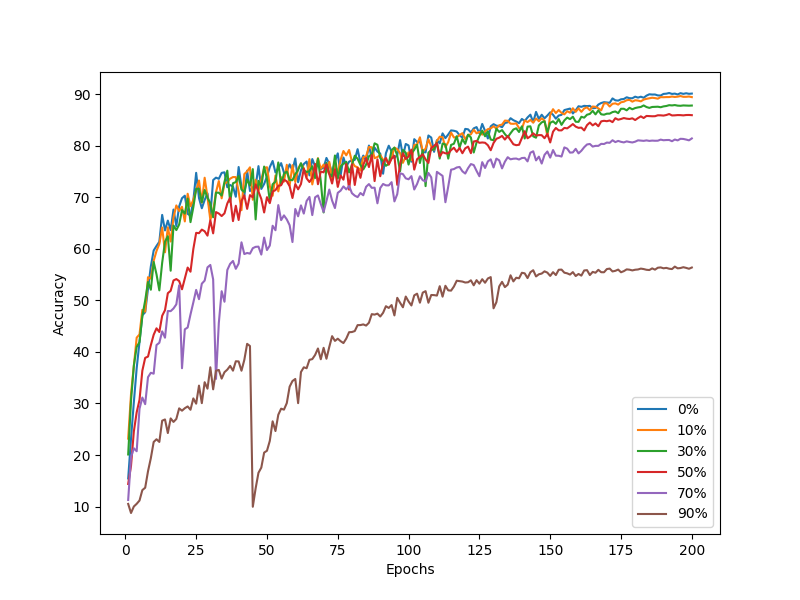
\includegraphics[width=1\linewidth]{fig_datadistill/cifar_results_nearest.png}
    % \caption{Accuracy over Epochs of training for ResNet-50 Classifiers trained on the CIFAR-10 dataset with different levels of Clustering-Based DD}
    \label{fig:cifar_results_nearest}
\end{figure}


\begin{figure}
    \centering
    \caption[Accuracy on CIFAR-10 using removal on furthest distance to cluster centroid]{Accuracy over Epochs of training for ResNet-50 Classifiers trained on the CIFAR-10 dataset with different levels of Clustering-Based DD. The removal criterion used was Furthest distance to cluster centroid.}
    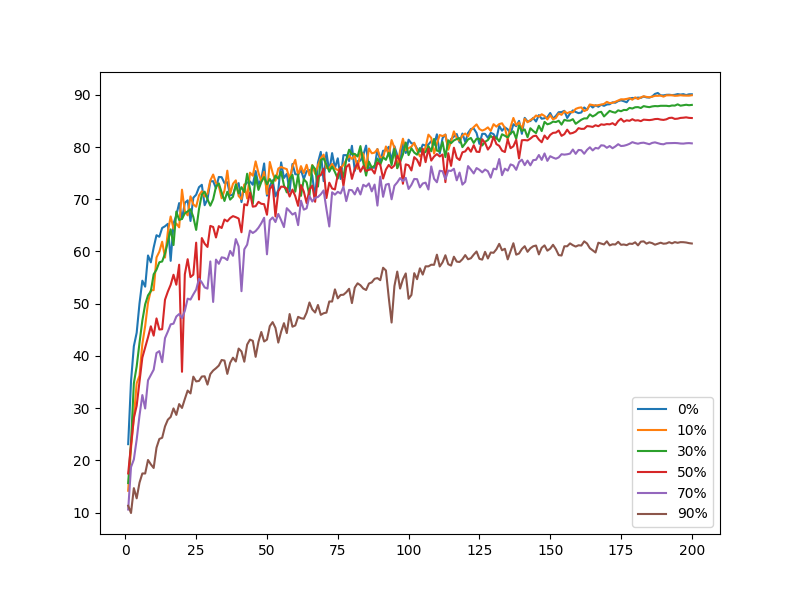
\includegraphics[width=1\linewidth]{fig_datadistill/cifar_results_furthest.png}
    % \caption{Accuracy over Epochs of training for ResNet-50 Classifiers trained on the CIFAR-10 dataset with different levels of Clustering-Based DD}
    \label{fig:cifar_results_furthest}
\end{figure}


\begin{figure}
    \centering
    \caption[Accuracy on CIFAR-10 using random sample removal]{Accuracy over Epochs of training for ResNet-50 Classifiers trained on the CIFAR-10 dataset with different levels of Clustering-Based DD. The removal criterion used was Random sample removal}
    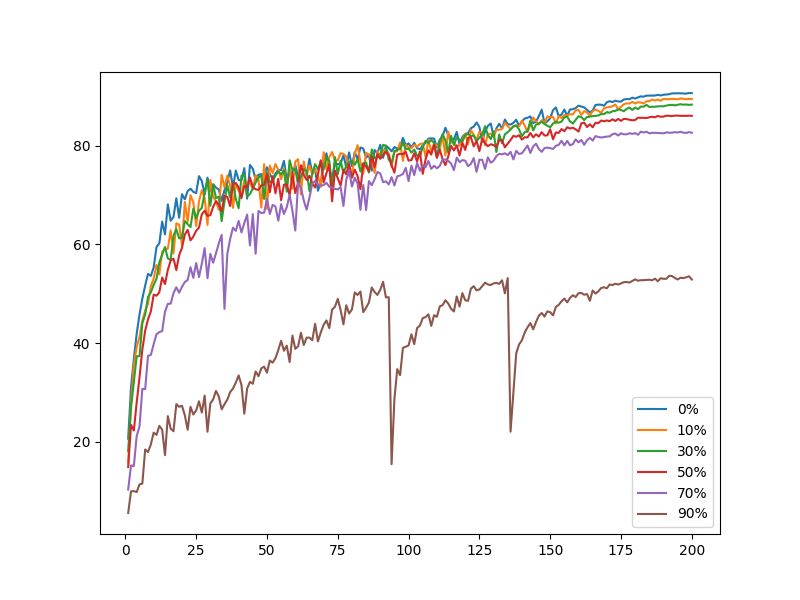
\includegraphics[width=1\linewidth]{fig_datadistill/cifar_results_random.png}
    % \caption{Accuracy over Epochs of training for ResNet-50 Classifiers trained on the CIFAR-10 dataset with different levels of Clustering-Based DD}
    \label{fig:cifar_results_random}
\end{figure}

The effect of our Clustering-Based DD method on the data's global structure was also investigated. This was done by using UMAP \cite{mcinnes2018umap} to perform dimension reduction on the dataset in order to be able to represent certain classes as 2D heatmap plots. This process was repeated at different levels of DD, and using Random, Nearest and Furthest distance criteria for data sample removal. Figure \ref{fig:cifar_0_heatmaps} shows the UMAP heatmap visualizations of CIFAR-10 class 0 (airplane), and Figure \ref{fig:cifar_1_heatmaps} shows them for CIFAR-10 class 1 (automobile). 


\begin{figure}[t]
    \caption[CIFAR-10 Class 0 (airplane) represented as a 2D heatmap using UMAP]{CIFAR-10 Class 0 (airplane) represented as a 2D heatmap using UMAP, at different levels of DD using Random, Nearest, and Furthest cluster distance criteria}
    \subfigure[Random Sample Removal - 0\% DD]{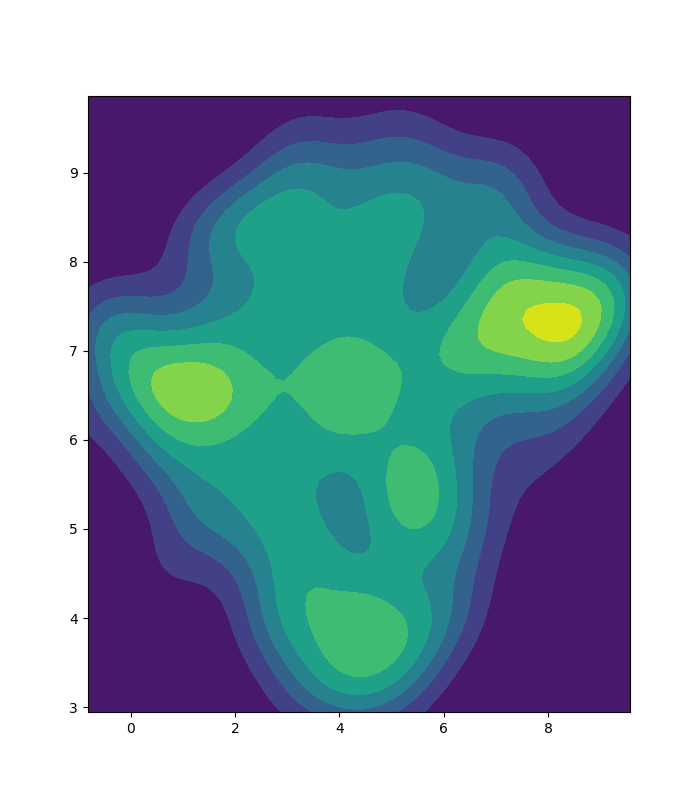
\includegraphics[width=0.33\linewidth]{fig_datadistill/cifar_class_0_random_vis_prop_0.png}}
    \subfigure[Random Sample Removal - 50\% DD]{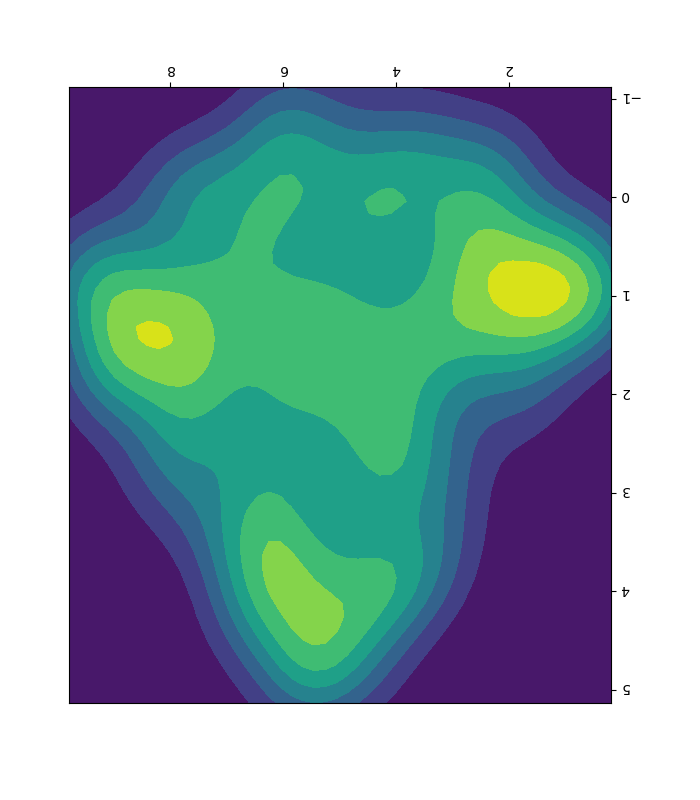
\includegraphics[width=0.33\linewidth]{fig_datadistill/cifar_class_0_random_vis_prop_5.png}}
    \label{fig:ALLVITS}
    \subfigure[Random Sample Removal - 90\% DD]{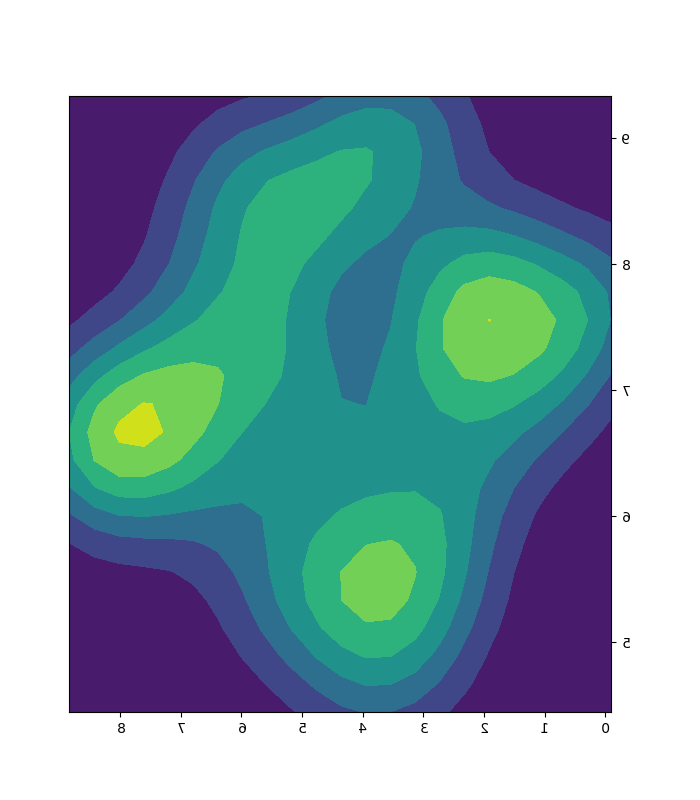
\includegraphics[width=0.33\linewidth]{fig_datadistill/cifar_class_0_random_vis_prop_9.png}}
    \subfigure[Nearest Sample Removal - 0\% DD]{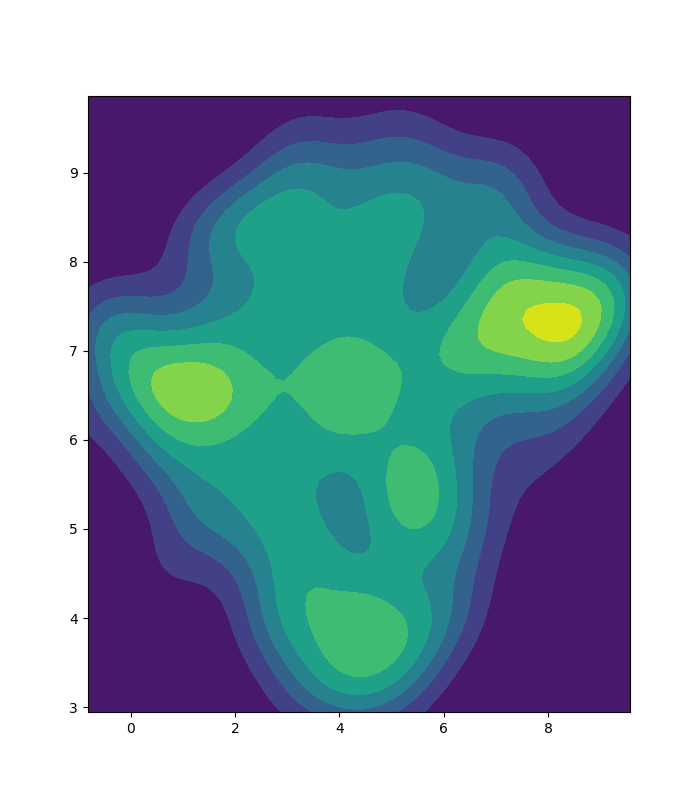
\includegraphics[width=0.33\linewidth]{fig_datadistill/cifar_class_0_nearest_vis_prop_9.png}}
    \subfigure[Nearest Sample Removal - 50\% DD]{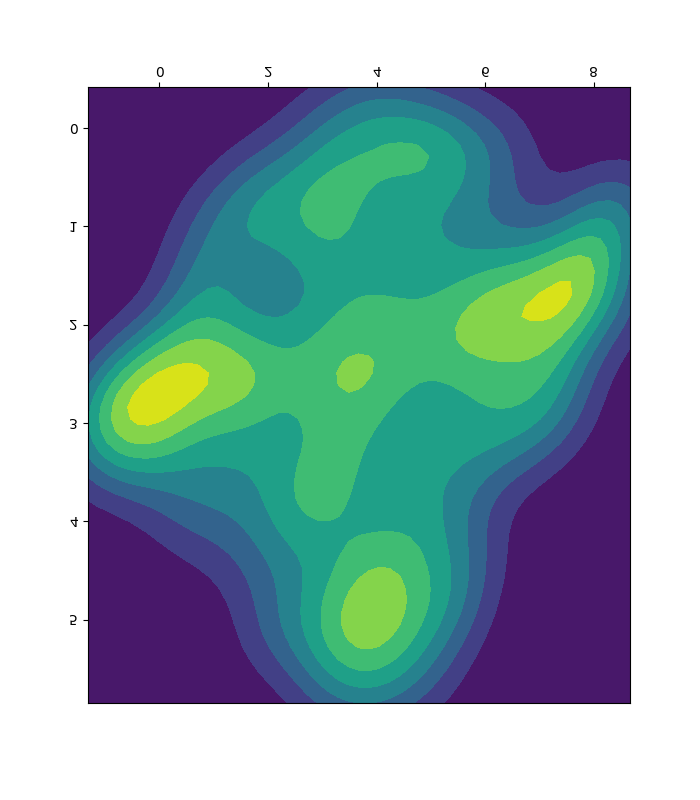
\includegraphics[width=0.33\linewidth]{fig_datadistill/cifar_class_0_nearest_vis_prop_5.png}}
    \label{fig:ALLVITS}
    \subfigure[Nearest Sample Removal - 90\% DD]{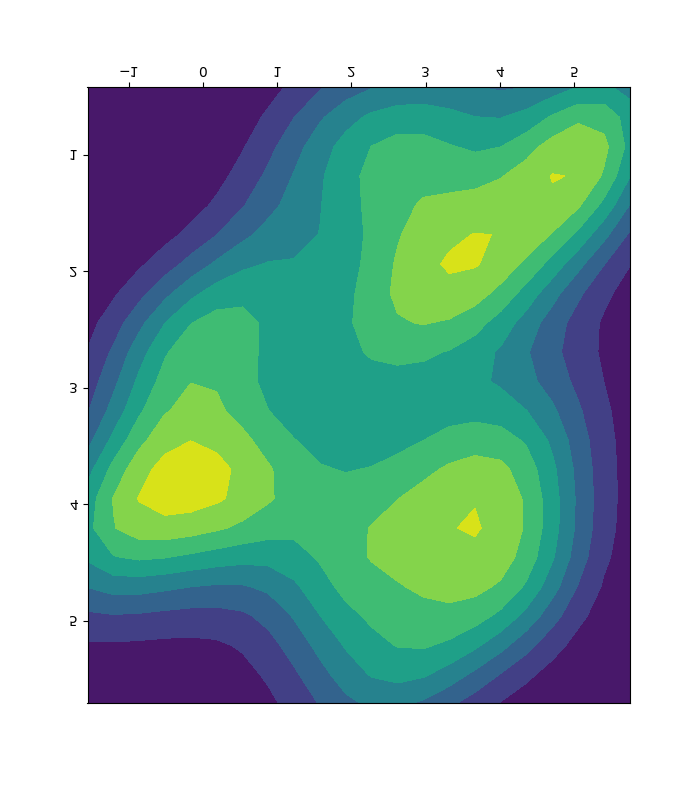
\includegraphics[width=0.33\linewidth]{fig_datadistill/cifar_class_0_nearest_vis_prop_0.png}}   
    \subfigure[Furthest Sample Removal - 0\% DD]{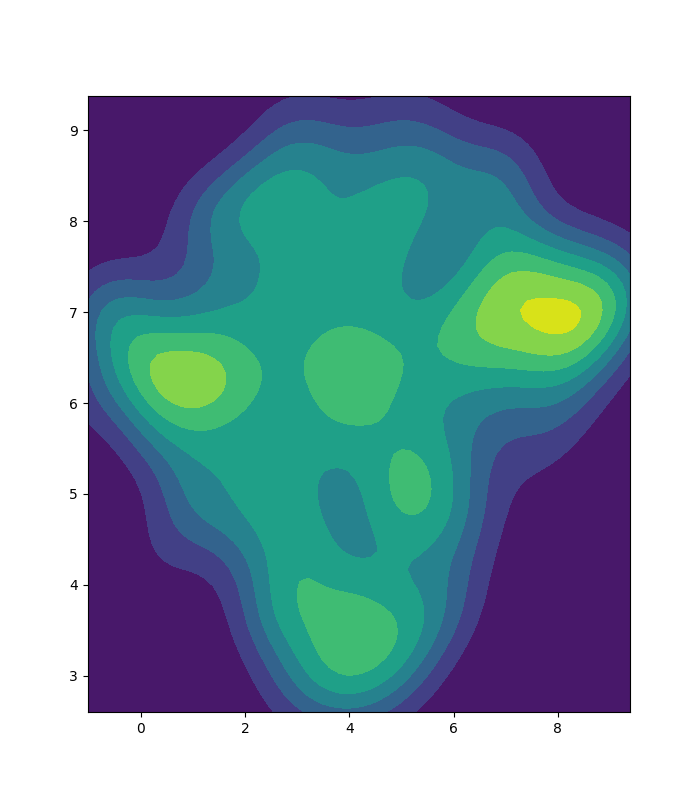
\includegraphics[width=0.33\linewidth]{fig_datadistill/cifar_class_0_furthest_vis_prop_0.png}}
    \subfigure[Furthest Sample Removal - 50\% DD]{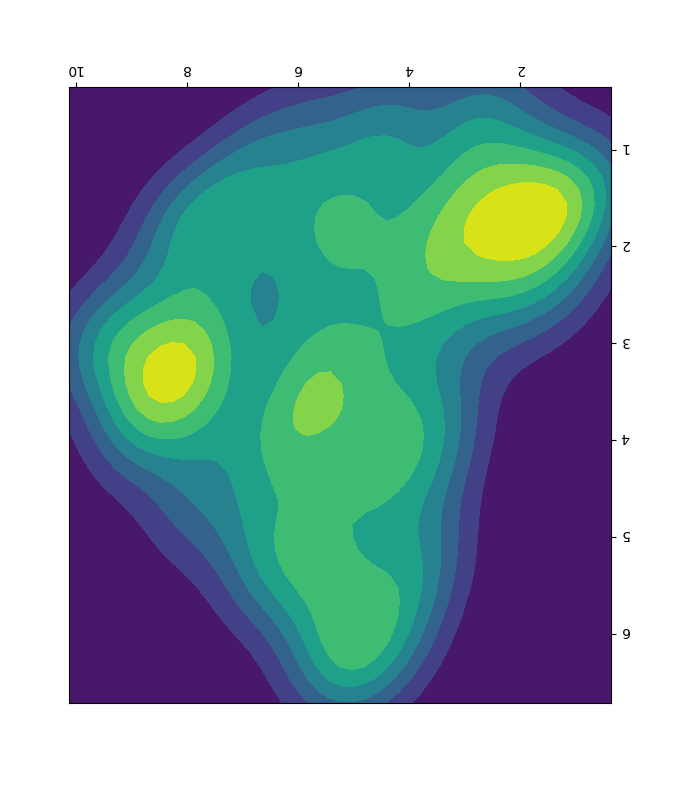
\includegraphics[width=0.33\linewidth]{fig_datadistill/cifar_class_0_furthest_vis_prop_5.png}}
    \label{fig:ALLVITS}
    \subfigure[Furthest Sample Removal - 90\% DD]{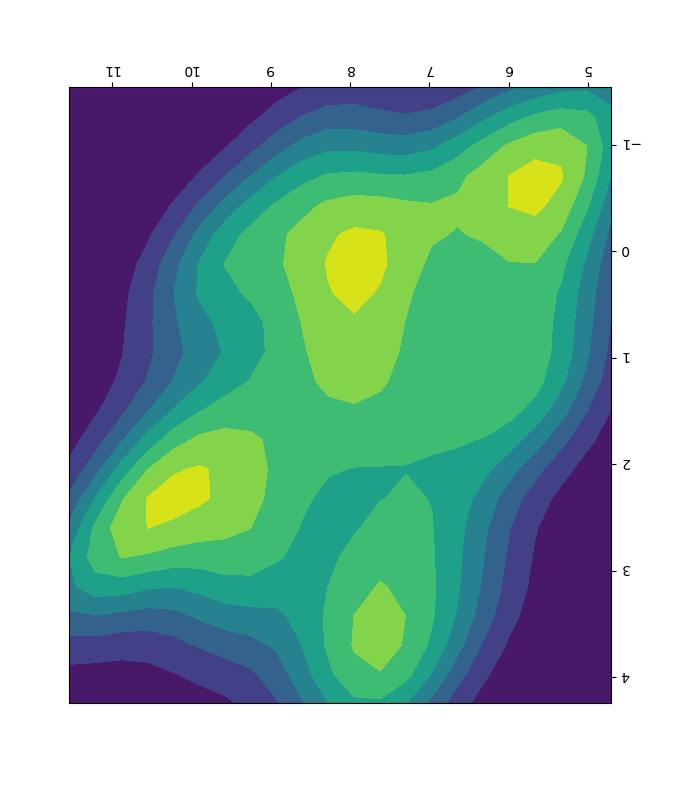
\includegraphics[width=0.33\linewidth]{fig_datadistill/cifar_class_0_furthest_vis_prop_9.png}}
    % \caption{CIFAR-10 Class 0 (airplane) represented as a 2D heatmap using UMAP, at different levels of DD using Random, Nearest, and Furthest cluster distance criteria}
    \label{fig:cifar_0_heatmaps}
\end{figure}


\begin{figure}[t]
    \caption[CIFAR-10 Class 1 (automobile) represented as a 2D heatmap using UMAP]{CIFAR-10 Class 1 (automobile) represented as a 2D heatmap using UMAP, at different levels of DD using Random, Nearest, and Furthest cluster distance criteria}
    \subfigure[Random Sample Removal - 0\% DD]{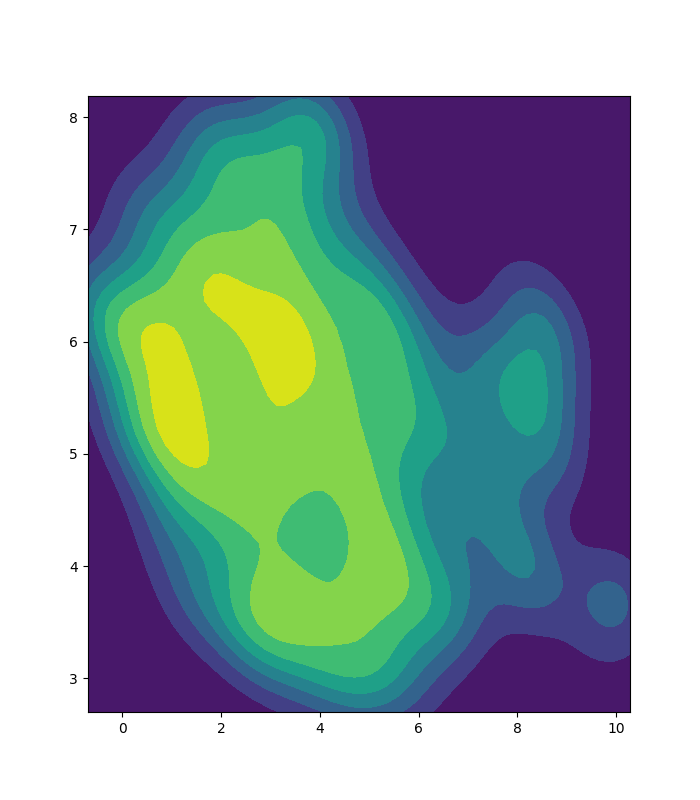
\includegraphics[width=0.33\linewidth]{fig_datadistill/cifar_class_1_random_vis_prop_0.png}}
    \subfigure[Random Sample Removal - 50\% DD]{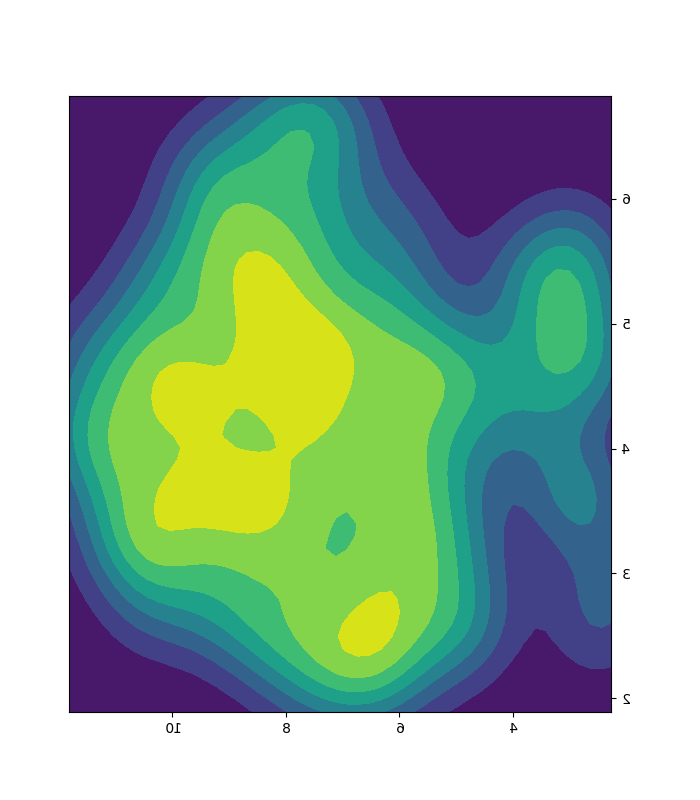
\includegraphics[width=0.33\linewidth]{fig_datadistill/cifar_class_1_random_vis_prop_5.png}}
    \label{fig:ALLVITS}
    \subfigure[Random Sample Removal - 90\% DD]{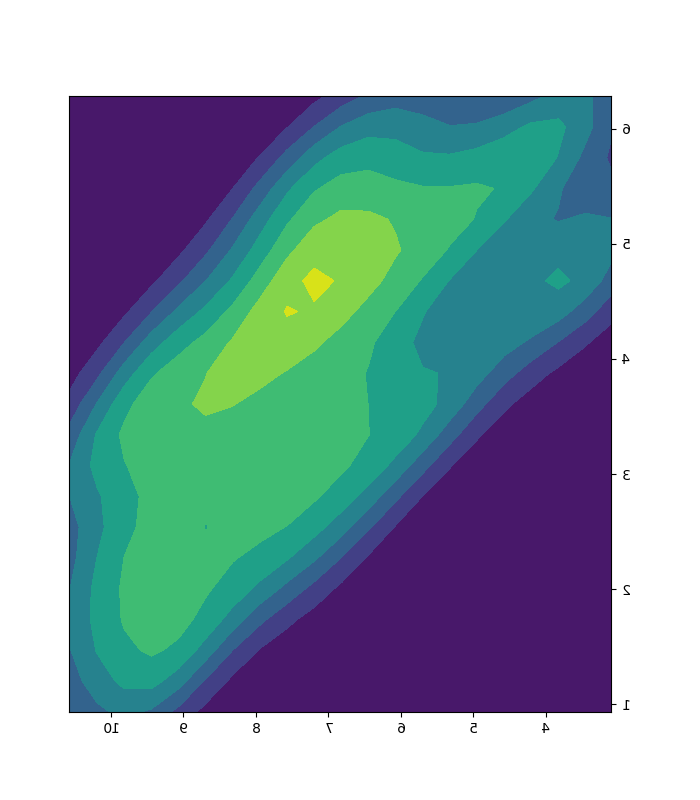
\includegraphics[width=0.33\linewidth]{fig_datadistill/cifar_class_1_random_vis_prop_9.png}}
    \subfigure[Nearest Sample Removal - 0\% DD]{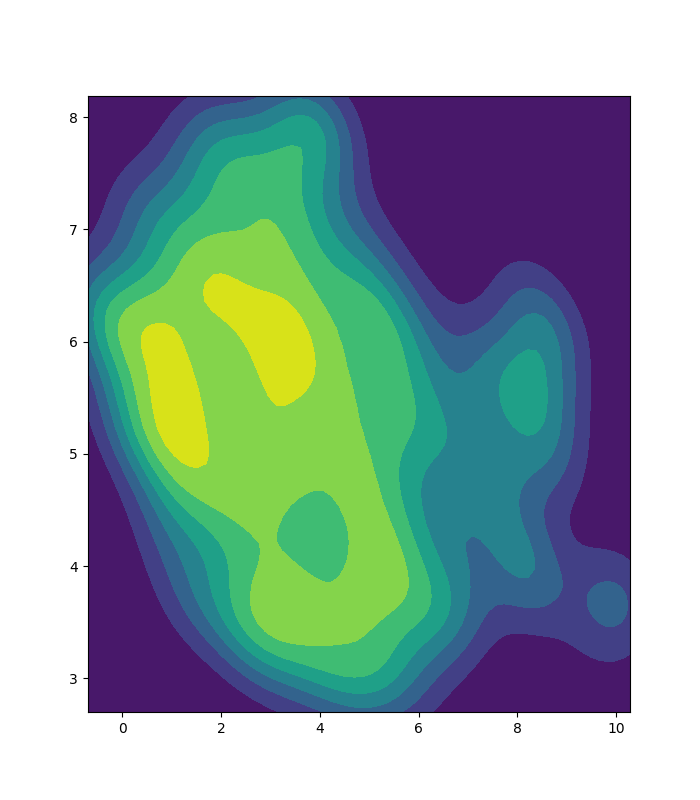
\includegraphics[width=0.33\linewidth]{fig_datadistill/cifar_class_1_nearest_vis_prop_9.png}}
    \subfigure[Nearest Sample Removal - 50\% DD]{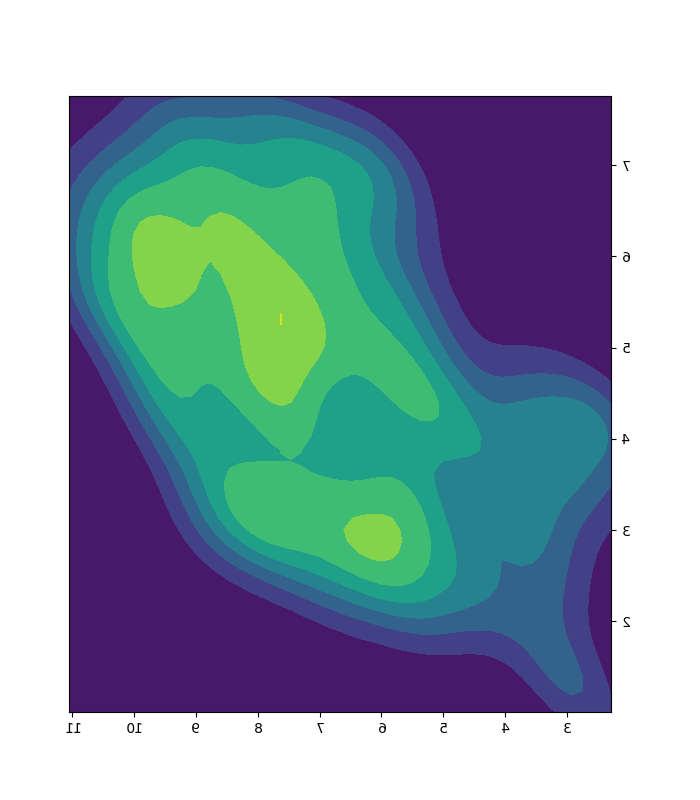
\includegraphics[width=0.33\linewidth]{fig_datadistill/cifar_class_1_nearest_vis_prop_5.png}}
    \label{fig:ALLVITS}
    \subfigure[Nearest Sample Removal - 90\% DD]{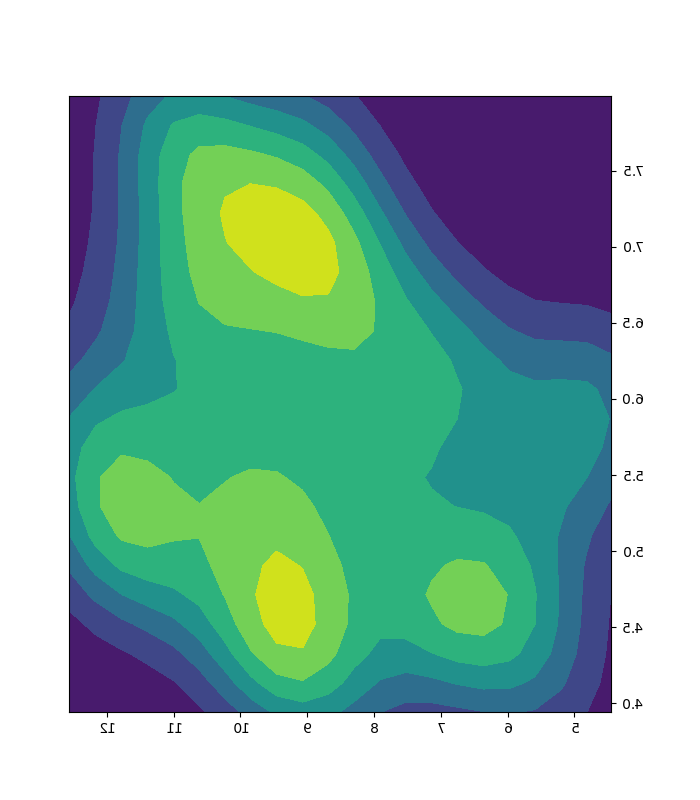
\includegraphics[width=0.33\linewidth]{fig_datadistill/cifar_class_1_nearest_vis_prop_0.png}}    
    \subfigure[Furthest Sample Removal - 0\% DD]{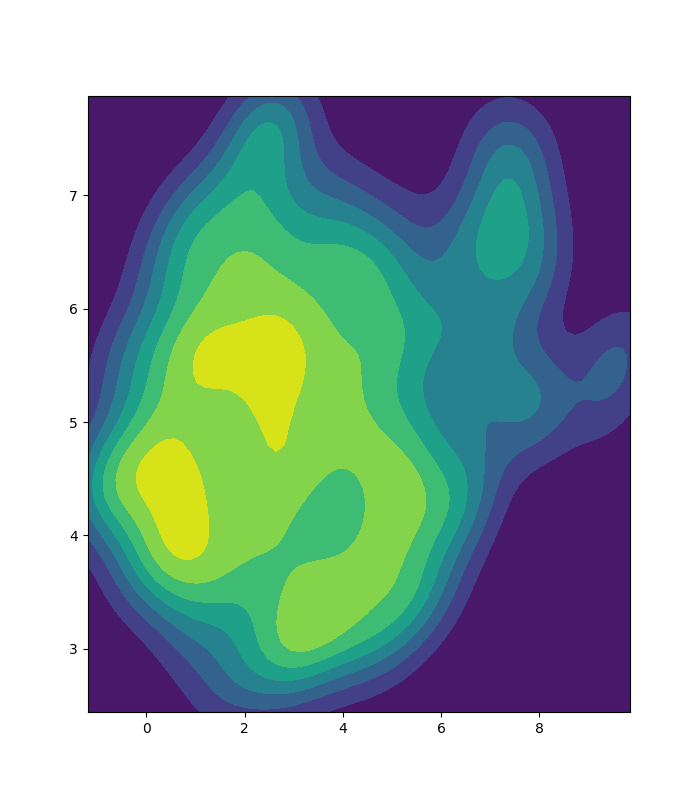
\includegraphics[width=0.33\linewidth]{fig_datadistill/cifar_class_1_furthest_vis_prop_0.png}}
    \subfigure[Furthest Sample Removal - 50\% DD]{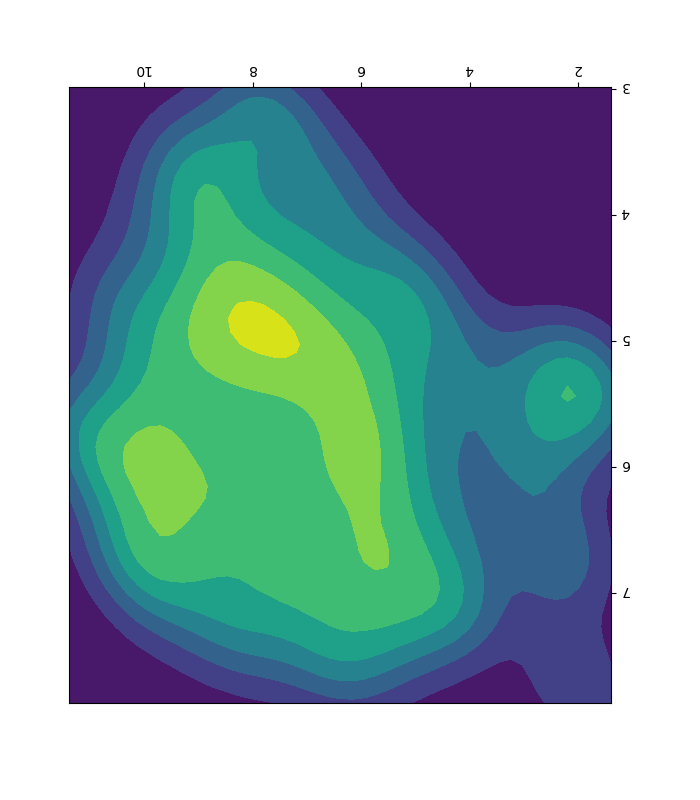
\includegraphics[width=0.33\linewidth]{fig_datadistill/cifar_class_1_furthest_vis_prop_5.png}}
    \label{fig:ALLVITS}
    \subfigure[Furthest Sample Removal - 90\% DD]{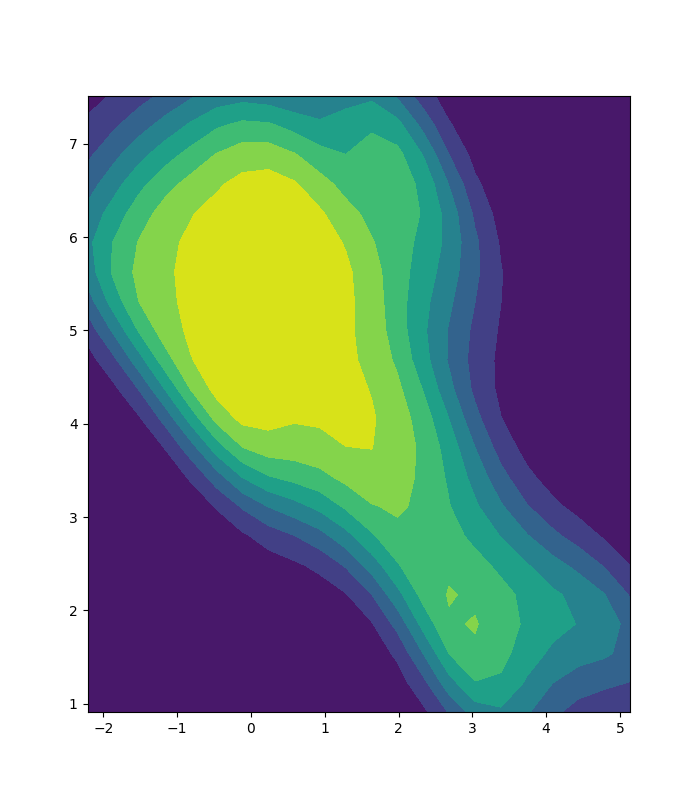
\includegraphics[width=0.33\linewidth]{fig_datadistill/cifar_class_1_furthest_vis_prop_9.png}}
    % \caption{CIFAR-10 Class 1 (automobile) represented as a 2D heatmap using UMAP, at different levels of DD using Random, Nearest, and Furthest cluster distance criteria}
    \label{fig:cifar_1_heatmaps}
\end{figure}

Interpreting Figures \ref{fig:cifar_0_heatmaps} and \ref{fig:cifar_1_heatmaps}, we can see that while the Clustering-Based DD method is able to significantly reduce the size of image datasets, it also leads to a substantial shift in the underlying structure of the data. For both classes 0 and 1, we can observe that 90\% DD fundamentally changes the shape of the data structure with all three distance criteria. However, when we look at the UMAP visualizations for the 50\% DD, there are certain distance criteria affect the data structure more than others. In the case of Random Sample Removal at 50\% DD (Figures \ref{fig:cifar_0_heatmaps}(b) and \ref{fig:cifar_1_heatmaps}(b)), the heatmaps do not change a lot from their respective baselines (Figures \ref{fig:cifar_0_heatmaps}(a) and \ref{fig:cifar_1_heatmaps}(a)), while for Nearest (Figures \ref{fig:cifar_0_heatmaps}(e) and \ref{fig:cifar_1_heatmaps}(e)) and Furthest Sample Removal at 50\% DD (Figures \ref{fig:cifar_0_heatmaps}(h) and \ref{fig:cifar_1_heatmaps}(5)), the heatmap shapes deviate significantly from those of the baseline. This indicates that the Clustering-Based DD method also changes the distribution of the data after distillation is performed.

\subsubsection{Conclusion and Future Work}

The experimental results achieved for the MNIST and CIFAR-10 datasets indicate that our Clustering-Based DD method can significantly reduce the size of image datasets while causing a relatively small loss in classification accuracy. In the case of the MNIST dataset, we achieved a 50\% decrease in dataset size while losing less than 0.4\% model accuracy compared to the baseline, and for the CIFAR-10 dataset, the accuracy loss at 50\% distillation was just 4.19\% compared to the baseline (Table \ref{tab:dataset_distillation_results}). These are promising initial results, especially with our current basic clustering method. 

In addition to our method's adherence to MANOLO's project goal of improved efficiency for AI techniques, the use of Clustering-Based DD also meets MANOLO's criteria for ethicism and modality agnosticism. Due to the fact that we only require the use of the dataset's latent space for the distillation process, there is no need for the transfer of sensitive or private user data - the clustering can be completed on the user or edge device, and only the encoded latent space needs to be transferred to MANOLO. Also, as mentioned in Section \ref{introduction}, our DD methodology is compatible with computing paradigms that are not compatible with more traditional DD techniques, specifically Neuromorphic Computing.

Further work in this area will explore the use of more complex clustering approaches. While K-means clustering has a number of benefits that are in line with MANOLO's project goals, it is important that the shape of the data distribution is kept the same before and after the distillation process. Examining the UMAP heatmaps (Figures \ref{fig:cifar_0_heatmaps} and \ref{fig:cifar_1_heatmaps}) generated of the CIFAR-10 dataset before and after the application of the Clustering-Based DD method, it's clear that in its current iteration, the technique does not sufficiently preserve the underlying data distribution. A more sophisticated, hybrid approach will be employed in the future to attempt to alleviate this problem, rather than just distilling based on the points' distance to cluster centroids.
